\documentclass [a4paper] {report}
\usepackage{amsmath,amssymb,amsthm, bbm, graphicx,listings,braket,subfig,titlesec,cleveref,lipsum,mcode,xcolor-patch, textcomp,float,booktabs,siunitx, listings}
\usepackage[authoryear]{natbib}
\usepackage[section]{placeins}
\usepackage[margin=2.2cm]{geometry}
\titleformat{\chapter}{\normalfont\huge}{\thechapter.}{20pt}{\huge \bf}

\DeclareMathOperator*{\argmin}{arg\,min}
\DeclareMathOperator*{\argmax}{arg\,max}
\newcommand{\norm}[1]{\left\lVert #1 \right\rVert}

\begin{document}
	
	\begin{titlepage}
		\begin{center}
			
			\textsc{\LARGE IN4320 Machine Learning}\\[1.25cm]
			
			\rule{\linewidth}{0.5mm}\\[1.0cm]
			{\huge \bfseries Exercises Regularization and Sparsity }\\[0.6cm]
			\rule{\linewidth}{0.5mm}\\[1.5cm]
			
			\begin{minipage}{0.4\textwidth}
				\begin{flushleft} \large	
					\emph{Author:}\\
					\textsc{Milan Niestijl, 4311728}
				\end{flushleft}
			\end{minipage}
			
			\vfill
			{\large \today}
		\end{center}
	\end{titlepage}
	
	\chapter*{Theory}
	\setcounter{page}{1}
	\pagenumbering{arabic}
	In these exercises, a regularized version of the nearest mean classifier (NMC) is considered for two-class data. We first develop some theory, which will help us answer the questions later on.\\
	Mathematically, the problem can be formulated as follows: Given $\lambda \in \mathbb{R}$, $N$ d-dimensional feature vectors $x_{i} \in \mathbb{R}^{d}$, $i \in \{ 1, 2, ..., N \}$ and their label $y_{i} \in {+,-}$, find $m_{-}, m_{+} \in \mathbb{R}^{d} $ such that the loss function $L$ is minimized:
	\begin{equation}
		L(m_{-},m_{+}) = \sum_{i=1}^{N} \norm{x_{i} - m_{y_{i}}}_{2}^{2} + \lambda \norm{m_{-} - m_{+}}_{1}
		\label{LossFunction1}
	\end{equation}
	The optimal solution is denoted by $(\hat{m}_{-},\hat{m}_{+})$. That is, 
	\begin{equation}
		(\hat{m}_{-},\hat{m}_{+}) = \argmin_{m_{-},m_{+}} L(m_{-},m_{+}) 
	\end{equation}
	In order to find the optimal solution, we note that the loss function can be decomposed in the following manner:
	\begin{equation}
		\begin{split}
			L(m_{-},m_{+}) &= \sum_{i=1}^{N} \norm{x_{i} - m_{-}}_{2}^{2} \mathbbm{1}_{\{y_{i}=-\}} + \sum_{i=1}^{N} \norm{x_{i} - m_{+}}_{2}^{2} \mathbbm{1}_{\{y_{i}=+\}}  + \lambda \norm{m_{-} - m_{+}}_{1} \\
			&= L_{-}(m_{-}) + L_{+}(m_{+}) + \lambda L_{1}(m_{-},m_{+})			
		\end{split}
	\end{equation}
	Where:
	\begin{equation}
		\begin{split}
			& L_{-}(m_{-}) = \sum_{i=1}^{N} \norm{x_{i} - m_{-}}_{2}^{2} \mathbbm{1}_{\{y_{i}=-\}}\\
			& L_{+}(m_{+}) = \sum_{i=1}^{N} \norm{x_{i} - m_{+}}_{2}^{2} \mathbbm{1}_{\{y_{i}=+\}}\\
			& L_{1}(m_{-},m_{+}) = \norm{m_{-} - m_{+}}_{1}
		\end{split}
	\end{equation}
	
	\noindent
	We now proceed to find the optimal solution. Let $j \in \{1,2, ..., d \}$. In order to calculate the partial derivatives $\frac{\partial L}{\partial(m_{-})_{j}}$ and $\frac{\partial L}{\partial(m_{+})_{j}}$, we assume $(m_{-})_{j} \neq (m_{+})_{j}$. Let $n$, $k>0$ be the number of $-$ and $+$ labels, respectively. We have:
	\begin{equation}
		\begin{split}
			\frac{\partial L}{\partial(m_{-})_{j}} &= 2n m_{-} - 2 \sum_{i=1}^{N} x_{ij} \mathbbm{1}_{\{y_{i}=-\}} + \frac{\lambda (m_{-} - m_{+})_{j}}{|(m_{-} - m_{+})_{j}|}\\
			\frac{\partial L}{\partial(m_{+})_{j}} &= 2k m_{+} - 2 \sum_{i=1}^{N} x_{ij} \mathbbm{1}_{\{y_{i}=+\}} - \frac{\lambda (m_{-} - m_{+})_{j}}{|(m_{-} - m_{+})_{j}|}\\
		\end{split}		
	\end{equation}
	
	\noindent
	Setting the partial derivatives to zero and rearranging the terms, we find:	
	\begin{equation}
		\begin{split}
			(m_{-})_{j} > (m_{+})_{j} \implies 
				\begin{cases}
					(\hat{m}_{-})_{j} = \overline{(m_{-})_{j}} - \frac{1}{2n}\lambda\\
					(\hat{m}_{+})_{j} = \overline{(m_{+})_{j}} + \frac{1}{2k}\lambda
				\end{cases}\\
			(m_{-})_{j} < (m_{+})_{j} \implies 
				\begin{cases}
					(\hat{m}_{-})_{j} = \overline{(m_{-})_{j}} + \frac{1}{2n}\lambda\\
					(\hat{m}_{+})_{j} = \overline{(m_{+})_{j}} - \frac{1}{2k}\lambda
				\end{cases}
		\end{split}
		\label{solution1}
	\end{equation}
	Where $\overline{(m_{-})_{j}} = \frac{1}{n} \sum_{i=1}^{N} x_{ij} \mathbbm{1}_{\{y_{i}=-\}}$ and $\overline{(m_{+})_{j}} = \frac{1}{k} \sum_{i=1}^{N} x_{ij} \mathbbm{1}_{\{y_{i}=+\}}$.\\\\
	Thus, for both partial derivatives to be simultaneously to be zero, we require $\hat{m}_{-} \geq \hat{m}_{+}$ or $\hat{m}_{-} \leq \hat{m}_{+}$, respectively, in which case the optimal solution $(\hat{m}_{-},\hat{m}_{+})_{j}$ is given by equation \ref{solution1}. This requirement can be reformulated as:
	\begin{equation}
		|\overline{(m_{-})_{j}} - \overline{(m_{+})_{j}}| \geq \lambda \left(\frac{1}{2n} + \frac{1}{2k}\right)
		\label{condition}
	\end{equation}
	If this condition is not met, then there is no point at which both partial derivatives are simultaneously zero. We proceed and assume no such point exists. As the loss function $L$ is convex, a (global) minimum does exist. Since there is no point at which the gradient is zero, it follows that the derivative is not defined at the minimum. Hence, we must have $(m_{-})_{j} = (m_{+})_{j} =: (m)_{j}$, so that the contribution of the $j^{th}$ coordinate to the loss function is just $\sum_{i=1}^{N} |(x_{i} - m)_{j}|^{2}$. This is clearly minimized by the average of the $j^{th}$ coordinate of the training data:
	\begin{equation}
		(\hat{m})_{j} = (\hat{m}_{-})_{j} = (\hat{m}_{+})_{j} = \frac{1}{N}\sum_{i=1}^{N}x_{ij}
		\label{solution2}
	\end{equation}
	\noindent
	We conclude that if condition \ref{condition} is met, then $(\hat{m}_{-},\hat{m}_{+})_{j}$ is given by equation \ref{solution1}. If on the other hand the condition is not met, then it is given by equation \ref{solution2}.
	
	{\let\clearpage\relax\chapter*{Exercises}}
	
	\section*{1.}
	\subsection*{a}
	The loss function $L(m_{+})$ is plotted for $\lambda \in \{0,2,4,6\}$ in figure \ref{fig:loss1}
	\begin{figure}[H]
		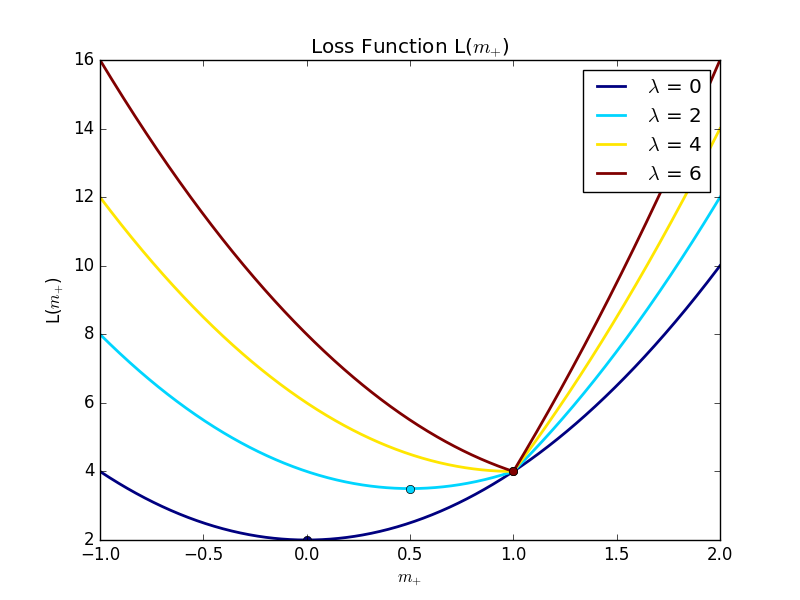
\includegraphics[scale=0.7]{Images/loss_function1.png}
		\caption{Loss function $L(m_{+})$ for various values of $\lambda$, using $d=1$, $m_{-}=1, x_{1} = 1, x_{2} = -1$ and $y_{1} = y_{2} = +$. The dots indicate the minimum of the function.}
		\label{fig:loss1}
	\end{figure}
	
	\subsection*{b}
	Fixing $m_{-}=1$, $\overline{m_{+}} = 0$, $n=0$ and $k=2$, condition \ref{condition} reduces to $\lambda<4$. Hence for $\lambda \in \{0,2\}$, there exists a point where the derivative equals zero, namely the point $\hat{m_{+}}=\frac{\lambda}{4}$. This point is thus the minimizer for $\lambda \in \{0,2\}$. For $\lambda \in \{4,6\}$, there is no point where the derivative equals zero, but the minimizer must satisfy $m_{+} = m_{-}$, hence $m_{+} = 1$. The minimum values are now easily calculated using the loss function. The result is shown in table \ref{table:loss_function}.
	
	\begin{table}[H]		
		\centering
		\caption{Overview of the minimizer and minimum value of the loss function $L(m_{+})$ for various $\lambda$.}
		\label{table:loss_function}
		\begin{tabular}{l c r}
			$\lambda$ &  $\hat{m_{+}}$  & $L(\hat{m_{+}})$ \\
			\hline
			0 & 0   & 2 \\
			2 & 0.5 & 3.5 \\
			4 & 1   & 4 \\
			6 & 1   & 4 \\
		\end{tabular}
	\end{table}
	
	\section*{2.}
	\subsection*{a}
	In general, the regularizer induces a bias towards the line $m_{-} = m_{+}$. That is, for increasing $\lambda$ the minimizer moves along the line that projects the unregularized $(\lambda=0)$ minimizer onto the line $m_{-} = m_{+}$. Thus, in the limiting behaviour $\lambda \rightarrow \infty$, the minimizer is given by this projection onto the line $m_{-} = m_{+}$.
	\subsection*{b}
	A contour line for the general loss function $L$ consists of a concatenation of two ellipses that intersect on the line $m_{-} = m_{+}$. A plot is shown in figure \ref{fig:contour}. It can be seen that the analytic minimizers, which are given by equations \ref{solution1} or \ref{solution2}, agree with the contour plot. Furthermore, the contour lines are "pulled" towards the line $m_{-} = m_{+}$ for increasing $\lambda$.
	\begin{figure}[H]
		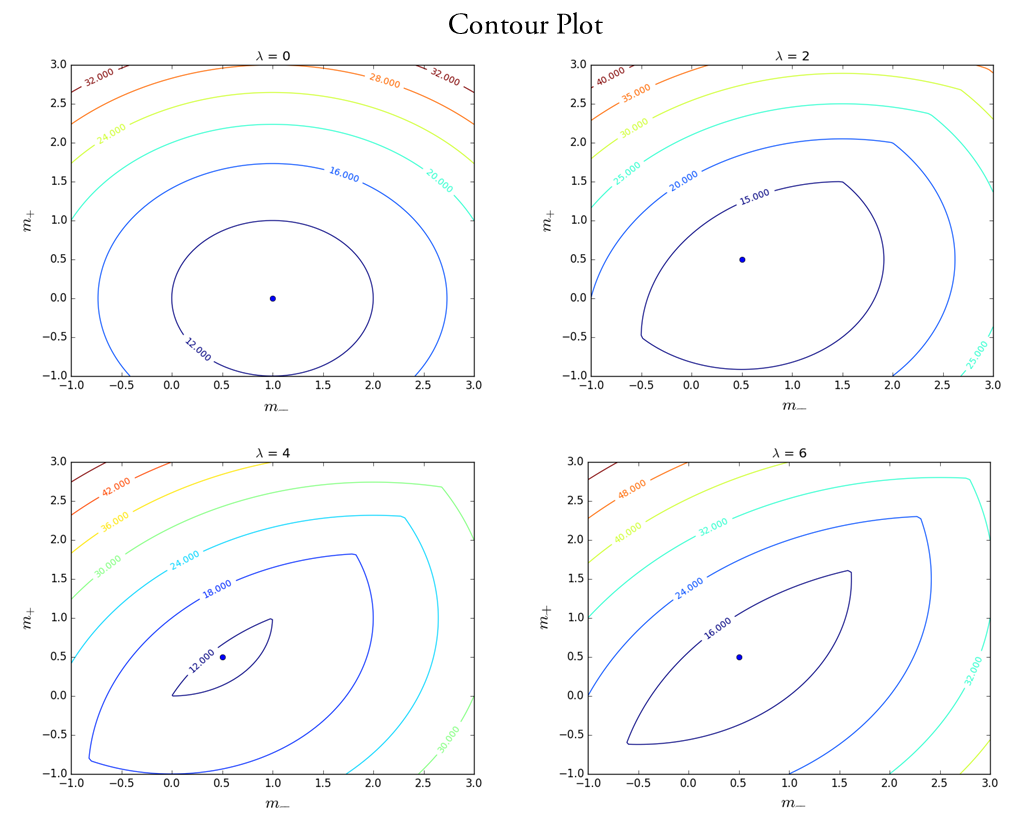
\includegraphics[width = \textwidth]{Images/contour_plot.png}
		\caption{Contour plot of $L(m_{-}, m_{+})$ for various values of $\lambda$ in the one-dimensional case. As data, $x = [-1,1,3,-1]$ and $y=[1,1,0,0]$ was used. The dots indicate the analytic minimizer of the loss function.}
		\label{fig:contour}
	\end{figure}
	\subsection*{c}
	The orthogonal projection of the point $(1,0)$ onto the line $m_{-} = m_{+}$ is given by $\left(\frac{1}{2}, \frac{1}{2}\right)$. Hence, for large enough $\lambda$, the solution $(\hat{m}_{-},\hat{m}_{+})$ will equal $\left(\frac{1}{2}, \frac{1}{2}\right)$.
	\section*{3.}
	\subsection*{a}
	The main ingredients of the optimization routine are explained in the theory part of this report. The actual implementation first separates the input data according to their class label, then checks using condition \ref{condition} for each dimension $j$ whether or not a point exists where both partial derivatives $\frac{\partial L}{\partial(m_{-})_{j}}$ and $\frac{\partial L}{\partial(m_{+})_{j}}$ equal zero. If so, it calculates $(\hat{m}_{-},\hat{m}_{+})_{j}$ according to equation \ref{solution1}. If not, then $(\hat{m}_{-},\hat{m}_{+})_{j}$ is calculated using equation \ref{solution2} instead. The (Python) code can be found at the end of the document.
	
	\subsection*{b}
	A plot for the two solution mean images for $\lambda=0$ and $\lambda$ large can be found in figure \ref{fig:image}. It can be seen that for large $\lambda$, the two image coincide, which is expected, as is explained in section \textbf{2.a}.
	\begin{figure}[H]
		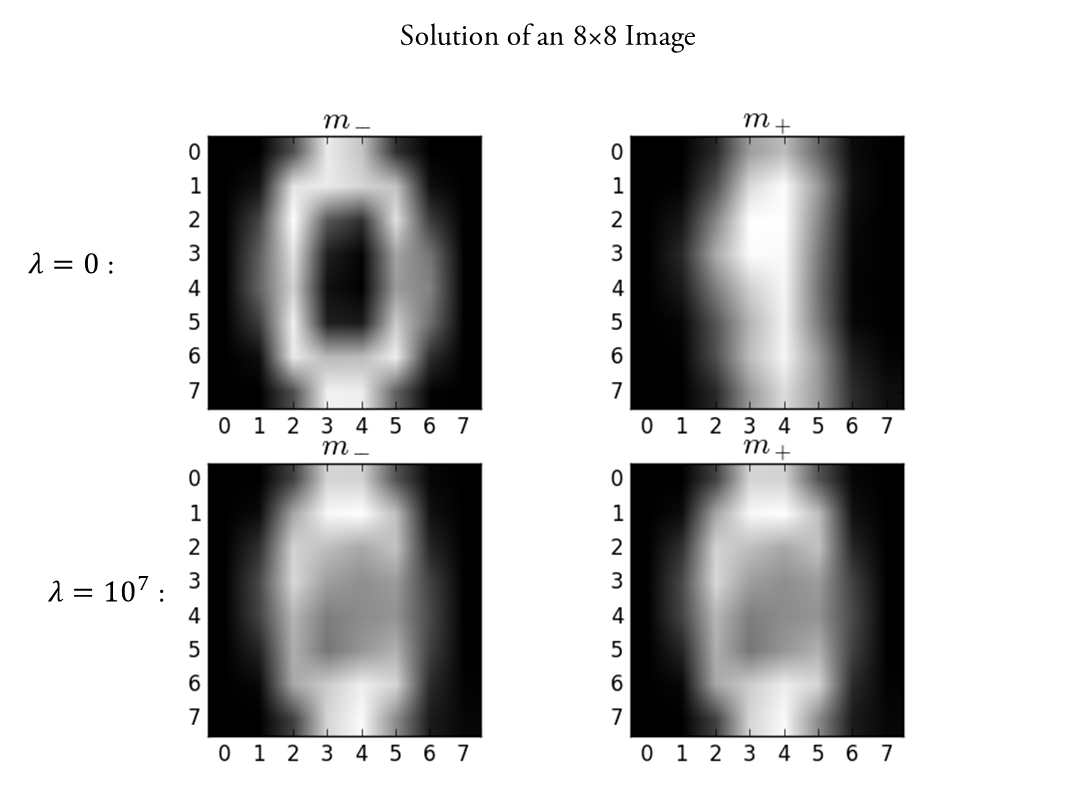
\includegraphics[width = \textwidth]{Images/figure_1.png}
		\caption{Image of the solution $(\hat{m}_{-},\hat{m}_{+})$ for $\lambda=0$ and $\lambda$ large. }
		\label{fig:image}
	\end{figure}
	\section*{Code:}
	\begin{lstlisting}
	class NMC():
		def __init__(self, Lambda):
			self.Lambda = Lambda
		
		# X ~ d*N, where d is the dimension of the data and N is the number of training samples.
		# y ~ N, classifying the i-th training example as 1 or 0, respectively.
		def fit(self, X, y):
			X0 = X[:,np.where(y==0)[0]]
			X1 = X[:,np.where(y==1)[0]]
			X0Mean = X0.mean(1)
			X1Mean = X1.mean(1)
			d = X.shape[0]
			n0 = X0.shape[1]
			n1 = X1.shape[1]
			M = np.zeros([d,2])
			for j in range(0,d):
				lambdaTerm = self.Lambda*(1/(2*n0) + 1/(2*n1))
				if (X0Mean[j] - X1Mean[j] >= lambdaTerm):
					M[j,0] = X0Mean[j] - self.Lambda/(2*n0)
					M[j,1] = X1Mean[j] + self.Lambda/(2*n1)
				elif (X1Mean[j] - X0Mean[j] >= lambdaTerm):
					M[j,0] = X0Mean[j] + self.Lambda/(2*n0)
					M[j,1] = X1Mean[j] - self.Lambda/(2*n1)
				else:
					M[j,[0,1]] = X[j,:].mean()
			self.M = M 
	\end{lstlisting}
	
	
\end{document}